\section{Results (provisional)}\label{sec:results}
\textbf{All numbers in this section are provisional, pending the owner's human labels.} They will be regenerated, in a fixed order (layer choice on the real validation set, temperature scaling, thresholds, then the head-to-head), once the labels exist.
\begin{table}[t]\centering\scriptsize
\caption{Layer comparison on the synthetic held-out validation split (15\% of the generated data). Mean = mean accuracy over the five decisions; $\star$ = kept. \textbf{PROVISIONAL -- pending human labels}.}
\label{tab:layers}\setlength{\tabcolsep}{3.5pt}
\begin{tabular}{lrrr rrr}\toprule
 & \multicolumn{3}{c}{Qwen2.5-0.5B (24 layers)} & \multicolumn{3}{c}{Qwen2.5-1.5B (28 layers)}\\
\cmidrule(lr){2-4}\cmidrule(lr){5-7}
Layer & Mean & R/C acc & R/C ECE & Mean & R/C acc & R/C ECE\\\midrule
12 & 91.6 & 92.9 & 0.052 & 91.2 & 93.6 & 0.063 \\
16 & 91.6 & 96.2 & 0.042 & 91.1 & 95.5 & 0.044 \\
20 & 91.6 & 94.9 & 0.043 & 91.7 & 96.2 & 0.043 \\
24 & 91.9 & 96.8 & 0.039 & 93.7 $\star$ & 97.4 & 0.030 \\
28 & n/a & n/a & n/a & 93.6 & 96.8 & 0.034 \\
mean 16--24 & 93.0 $\star$ & 95.5 & 0.045 & 93.4 & 95.5 & 0.041 \\
final (normed) & 92.2 & 96.8 & 0.037 & 93.2 & 96.8 & 0.031 \\
\bottomrule\end{tabular}\end{table}

\begin{table}[t]\centering\scriptsize
\caption{Per-class recall (\%) at the kept layer, synthetic held-out validation split. \textbf{PROVISIONAL -- pending human labels}.}
\label{tab:recall}\setlength{\tabcolsep}{3pt}
\begin{tabular}{l l p{4.6cm}}\toprule Decision & Model & Recall per class\\\midrule
Mode (direct / orchestrate) & 0.5B & direct 99, orchestrate 80 \\
Mode (direct / orchestrate) & 1.5B & direct 99, orchestrate 73 \\
Specialist & 0.5B & Frontend 71, Backend 75, DevOps \& Cloud 71, Security \& Compliance 80, QA \& Testing 91, Database 85, CTO Brain 81 \\
Specialist & 1.5B & Frontend 81, Backend 75, DevOps \& Cloud 89, Security \& Compliance 80, QA \& Testing 100, Database 85, CTO Brain 62 \\
Read / change & 0.5B & read 96, change 94 \\
Read / change & 1.5B & read 100, change 92 \\
QA gate & 0.5B & no 100, yes 91 \\
QA gate & 1.5B & no 95, yes 91 \\
Agent nature & 0.5B & technical 98, operational 99 \\
Agent nature & 1.5B & technical 97, operational 100 \\
\bottomrule\end{tabular}\end{table}

\subsection{Layers}
Table~\ref{tab:layers} compares layers on the synthetic validation split. Differences between layers are within about two points of mean accuracy; the mean of layers 16--24 is best for 0.5B and layer 24 for 1.5B. Specialist is the hardest decision (Table~\ref{tab:recall}).
\begin{table*}[t]\centering\scriptsize
\caption{Head-to-head on the held-out test split (strict independent truth), 3 repetitions. A case counts as correct when it is correct in the majority of its repetitions; 95\% Wilson intervals; exact McNemar test on the discordant cases ($b$ = only Jev right, $c$ = only the production LLM path right). Mode and QA gate: the production path is Claude; read/change: the production path is the local semantic router. \textbf{PROVISIONAL -- pending human labels}.}
\label{tab:h2h}
\begin{tabular}{l l r l l r r r}\toprule
Decision & Jev model & $n$ & Production path acc.\ \% [95\% CI] & Jev acc.\ \% [95\% CI] & $b/c$ & McNemar $p$ & Fallback \%\\\midrule
Mode (direct / orchestrate) & 0.5B & 39 & 100.0 [91.0, 100.0] & 100.0 [91.0, 100.0] & 0/0 & 1.000 & 5 \\
Read / change & 0.5B & 42 & 83.3 [69.4, 91.7] & 83.3 [69.4, 91.7] & 1/1 & 1.000 & 12 \\
QA gate & 0.5B & 7 & 71.4 [35.9, 91.8] & 71.4 [35.9, 91.8] & 0/0 & 1.000 & 100 \\
Mode (direct / orchestrate) & 1.5B & 39 & 100.0 [91.0, 100.0] & 100.0 [91.0, 100.0] & 0/0 & 1.000 & 5 \\
Read / change & 1.5B & 42 & 83.3 [69.4, 91.7] & 88.1 [75.0, 94.8] & 3/1 & 0.625 & 0 \\
QA gate & 1.5B & 7 & 71.4 [35.9, 91.8] & 71.4 [35.9, 91.8] & 0/0 & 1.000 & 100 \\
\bottomrule\end{tabular}\end{table*}

\begin{table*}[t]\centering\scriptsize
\caption{Read/change: Jev against a Claude classifier (plan login, same standing context and definition) and the production router. Strict = log-outcome truth with owner acceptance; extended = additional log rules for this decision only, lower confidence (Section~\ref{sec:truth}). McNemar against Claude. \textbf{PROVISIONAL -- pending human labels}.}
\label{tab:claude}
\begin{tabular}{l l r r l l r r}\toprule
Truth set & Jev & $n$ & Router \% & Claude \% [95\% CI] & Jev \% [95\% CI] & $b/c$ & McNemar $p$\\\midrule
strict & 0.5B & 42 & 83.3 & 73.8 [58.9, 84.7] & 83.3 [69.4, 91.7] & 5/1 & 0.219 \\
strict & 1.5B & 42 & 83.3 & 73.8 [58.9, 84.7] & 88.1 [75.0, 94.8] & 8/2 & 0.109 \\
strict + extended & 0.5B & 67 & 74.6 & 74.6 [63.1, 83.5] & 80.6 [69.6, 88.3] & 7/3 & 0.344 \\
strict + extended & 1.5B & 67 & 74.6 & 74.6 [63.1, 83.5] & 83.6 [72.9, 90.6] & 11/5 & 0.210 \\
\bottomrule\end{tabular}\end{table*}

\subsection{Held-out head-to-head}
On mode, the decider and the production path are both correct on all \nDone{} test cases; the set contains only one ``orchestrate'' case, and that class is off, so this result shows only that the decider answers ``direct'' cases correctly. On read/change (\nStrictDtwo{} cases), the 0.5B decider has the same accuracy as the router and the 1.5B decider is higher, but the difference is not significant (Table~\ref{tab:h2h}). Against the Claude classifier both deciders are higher, again without significance (Table~\ref{tab:claude}). Under the acceptance rule every measured result is \emph{non-inferior}; none is \emph{best}. The QA gate, specialist and agent-nature heads are off.
\begin{figure}[t]\centering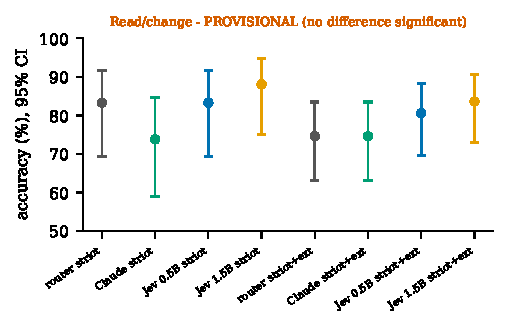
\includegraphics[width=\columnwidth]{figs/rc_acc.pdf}
\caption{Read/change accuracy with 95\% Wilson intervals. The intervals overlap; no difference is significant. \prov{}}\label{fig:rc}\end{figure}
\begin{figure}[t]\centering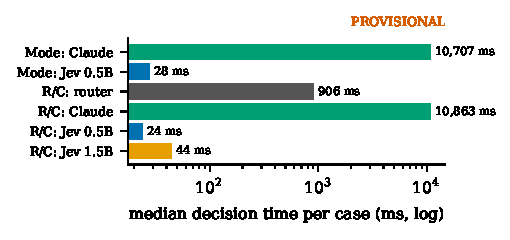
\includegraphics[width=\columnwidth]{figs/latency.pdf}
\caption{Median decision time per case (log scale). Mode: \dOneLlmMed{}\,s with Claude vs.\ \dOneJevMed{}\,ms with the decider. Read/change: \dTwoRouterMed{}\,ms router, \dTwoClaudeMed{}\,s Claude, \dTwoJevMed{}\,ms decider. \prov{}}\label{fig:lat}\end{figure}
\subsection{Calibration}
\begin{table}[t]\centering\scriptsize
\caption{Temperature scaling: ECE before ($T{=}1$) and after, on the synthetic validation split and on the real held-out test split. Target $<0.05$. \emph{off} = head disabled (fewer than 5 independent validation labels): the LLM decides. \textbf{PROVISIONAL -- pending human labels}.}
\label{tab:calib}\setlength{\tabcolsep}{2.5pt}
\begin{tabular}{l l r rr rr l}\toprule
 & & & \multicolumn{2}{c}{Synthetic val} & \multicolumn{2}{c}{Real test} & \\
\cmidrule(lr){4-5}\cmidrule(lr){6-7}
Model & Decision & $T$ & before & after & before & after & Head\\\midrule
0.5B & Mode (direct / orchestrate) & 6.76 & 0.032 & 0.026 & 0.000 & 0.007 & on \\
0.5B & Specialist & 5.58 & 0.195 & 0.064 & -- & -- & off \\
0.5B & Read / change & 5.07 & 0.045 & 0.017 & 0.126 & 0.090 & on \\
0.5B & QA gate & 9.93 & 0.042 & 0.069 & 0.571 & 0.544 & off \\
0.5B & Agent nature & 6.14 & 0.019 & 0.018 & -- & -- & off \\
1.5B & Mode (direct / orchestrate) & 9.93 & 0.036 & 0.054 & 0.000 & 0.014 & on \\
1.5B & Specialist & 4.60 & 0.143 & 0.037 & -- & -- & off \\
1.5B & Read / change & 4.60 & 0.030 & 0.030 & 0.098 & 0.153 & on \\
1.5B & QA gate & 13.26 & 0.066 & 0.070 & 0.000 & 0.247 & off \\
1.5B & Agent nature & 6.14 & 0.017 & 0.014 & -- & -- & off \\
\bottomrule\end{tabular}\end{table}

Temperature scaling reduces ECE on the synthetic validation split, mostly below the 0.05 target. On the real test split it does not reach the target and, for the 1.5B read/change head, makes it worse (Table~\ref{tab:calib}). A temperature fitted on generated data does not transfer to real messages; it will be refitted on the real validation set after the owner's labels. Until then Jev has no live authority (shadow mode).
\subsection{Real scenarios}
\begin{table*}[t]\centering\scriptsize
\caption{Real Odin scenarios on the isolated copy (same HTTP entry points as the desktop app), Normal vs.\ Jev mode, 2 complete paired repetitions (paused by the owner; one more run follows the re-measure on human labels). Jev used/fallback = decisions answered locally / handed to the LLM. Usage = reported plan usage per repetition, not charged. \textbf{PROVISIONAL -- pending human labels}.}
\label{tab:scen}
\begin{tabular}{l l r r r r r r r r}\toprule
Scenario & Mode & runs & reps & median s & mean s & mode acc.\ \% & Jev used/fallback & usage \$ & errors\\\midrule
Chat turn (routing) & normal & 12 & 2 & 35.3 & 46.3 & -- & 0/0 & 1.74 & 0 \\
Chat turn (routing) & jev & 12 & 2 & 20.4 & 37.4 & -- & 0/12 & 1.32 & 0 \\
Project run (mode) & normal & 6 & 2 & 124.0 & 128.0 & 100.0 & 0/0 & 2.72 & 0 \\
Project run (mode) & jev & 6 & 2 & 171.1 & 158.3 & 100.0 & 6/0 & 2.77 & 0 \\
\bottomrule\end{tabular}\end{table*}

Table~\ref{tab:scen} runs real owner requests through the same HTTP entry points as the desktop app, on an isolated copy of \sys{} in which remote tools are blocked. In the chat path the specialist head is off, so the router decides in both modes and the runs measure the decider's overhead when it falls back. In project runs the mode decision is made locally when the decider is confident. End-to-end time is dominated by the agents' own work and varies widely from run to run. In project runs the decider answered every mode decision locally (tens of milliseconds instead of about ten seconds), yet the Jev runs were not faster end to end: the saving is smaller than the run-to-run variation, and with two complete repetitions no end-to-end difference can be claimed in either direction. The chat-turn differences are also noise, since the router decided every chat turn in both modes. The third repetition stopped at a plan usage limit and is excluded from both modes in Table~\ref{tab:scen} until it is re-run.
\subsection{Where end-to-end time goes}
\begin{table}[t]\centering\scriptsize
\caption{Where end-to-end time goes in project runs: every available run (Normal 9 = 3 repetitions $\times$ 3 projects, Jev 6 = 2 $\times$ 3), split into LLM calls with the call ledger (start/end of every call). Mean / median seconds; turns = the agent's tool turns. \textbf{PROVISIONAL -- pending human labels}.}
\label{tab:timing}
\begin{tabular}{l r r}\toprule
Stage & Normal & Jev\\\midrule
Before the agent (mode + plan) & 17.5 / 16.3 & 10.1 / 10.2\\
\quad of which mode decision & one LLM call, 5--20\,s & 42--61\,ms (local)\\
Agent step & 113.6 / 118.4 & 119.8 / 123.7\\
\quad tool turns (mean / median) & 9.7 / 11 & 11 / 13.5\\
Review and answer & 26.4 / 20.7 & 31.5 / 30.3\\
Non-LLM time (\sys{} code, waits) & 0.5--0.9 & 0.5--0.7\\\midrule
\textbf{Total} & \textbf{154.5 / 154.7} & \textbf{158.3 / 171.1}\\
\bottomrule\end{tabular}\end{table}

Table~\ref{tab:scen} shows the Jev project runs 47\,s slower at the median. To find out why, every project run was split into its LLM calls using the call ledger, which records the start and end of every call; LLM time equals run time minus about 0.5\,s in every run, so the split is complete (Table~\ref{tab:timing}). Three findings follow. First, the 47\,s is the median of only the two paired repetitions; over every available run the gap is $+3.8$\,s in the mean, inside the run-to-run noise. Second, in every pair both modes took the same path (mode \emph{direct}, a one-step plan, the same agent), and Jev \emph{saves} about 7\,s before the agent because no mode-classifier LLM call is made. Third, the remaining difference is agent variance: the same agent on the same question took 49--217\,s and 3--19 tool turns within one mode (e.g.\ the Email agent in Normal mode: 81, 118 and 217\,s), and time follows the number of tool turns, not the mode. Per decision the decider is about 200 times faster (about 45\,ms against 5--20\,s), but end-to-end runs are dominated by the agents' own work, so with 6--9 runs no end-to-end gain can be measured yet; equally, Jev is not slower once the noise is accounted for. In shadow mode Jev cannot speed anything up by design. \prov{}
